 \documentclass[11pt]{article}
\usepackage{enumitem}
\usepackage{latexsym}
\usepackage{amsfonts}
\usepackage{amsmath,amssymb,amsthm}
\usepackage{xcolor}

\usepackage{tikz}
\usetikzlibrary{arrows}
\usetikzlibrary{automata}
\usetikzlibrary{positioning}


\setlength{\textheight}{8.5in}
\setlength{\textwidth}{6.0in}
\setlength{\headheight}{0in}
\addtolength{\topmargin}{-.5in}
\addtolength{\oddsidemargin}{-.5in}

\input{../lecture_notes/preamble.tex}


\newcommand{\solution}[1]{\paragraph{Solution}  }
\newcommand{\bl}[1]{\textcolor{blue}{#1}}
\newcommand{\rd}[1]{\textcolor{red}{#1}}

\begin{document}

\tikzset{
->, % makes the edges directed
>=stealth, % makes the arrow heads bold
node distance=2cm, % specifies the minimum distance between two nodes. Change if necessary.
every state/.style={thick, fill=gray!10}, % sets the properties for each ’state’ node
initial text=$ $, % sets the text that appears on the start arrow
}

\hw{1: Regular Languages}{1/13/2023}{}{Due:1/27/2023}

You should submit a typeset or \emph{neatly} written pdf on Canvas.  The grading TA should not have to struggle to read what you've written; if your handwriting is hard to decipher, you will be asked to typeset your future assignments. Five bonus points if you use \LaTeX, and our template. You may collaborate with other students, but any written work should be your own. 


\begin{enumerate}

    \item 
    
    One perspective of this class is that we are developing a theory of representation, or definability. For finite sets, this is easy, but it becomes more challenging for infinite languages. 

    \begin{enumerate}
        \item Prove every finite language is regular.
            \solution{}
            We can prove this in two ways: by creating a regular expression or by creating a DFA.

            \textbf{Regular Expression Proof}

            Let $L$ be a finite language. That is, $|L| = N$ is some finite value. Every word $w \in L$ is a regular expression since it is just a concatenation of some characters in $\Sigma$. Then the union of all of these words is also a regular expression since it is a finite union of regular expressions. This regular expression will only accept words if and only if they in the language. Thus, the language is regular.

            \textbf{DFA Proof}
            
            Let $L$ be a finite language. That is, $|L| = N$ is some finite value. To prove that $L$ is regular, we can create a NFA to decide it. For some string $w \in \Sigma^*$, let $w_i$ be the $i$-th character in the string. Now, we define an NFA as follows:

            \begin{enumerate}
                \item Create a start state
                \item For each word in the language $w \in L$, we create a chain from the start state, for which each action to the next state is the next character in the word. So, for each character $w_i$ in $w$, create a new state and connect it to the state for $w_{i - 1}$ (where $w_0$ is the start state). For this connection, use the action $w_i$. Then mark the last state for the word as a final accepting state.
            \end{enumerate}

            It should be clear that this NFA will accept a word if and only if the word is in the language since every word in the language is essentially "hard coded" into the NFA to be accepted and any other word will either not have a transition to go to or end in a non-accepting state.

            Note that since there are finite words in $L$ and every word within $L$ has a finite length, the number of states is finite. Now, since we have created an NFA for the language, we can use the process proven in lecture to convert it into a DFA that does the same computation, proving the language is regular. 
            
        \item Suppose we unrestricted our definition of DFA. We define a DIA to be exactly like a DFA except $|Q|=\infty$, and $\delta, F$ are adjusted appropriately. Prove that every language is decidable by a DIA.

            Now since we are allowed to have infinite states, we can apply the same method as from the DFA proof in (a) to "hard code" in every word within the language. Since we are now allowed infinite states, we can do this for an infinite amount of words, which may be required to decide an arbitrary language. Every language is a set of words, and now our NIA (or converted DIA) will accept all the words in the language, but no other word.
    
    \end{enumerate}
    
    \item Give an NFA, DFA, and regular expression for the following languages. Your NFA must be different than your DFA. Your solution doesn't have to be minimal, but it may assist the TA in grading. 
    \begin{itemize}
        \item $\{w \in \Sigma^* ~|~ w\text{ ends with } abba\}$
        \item $\{w \in \Sigma^* ~|~ w\text{ has a single b in the 3rd place from the right}\}$
    \end{itemize}

    \solution{} -
    \newline \newline
    $\{w \in \Sigma^* ~|~ w\text{ ends with } abba\}$

    NFA:
    \begin{figure}[ht]
        \centering
        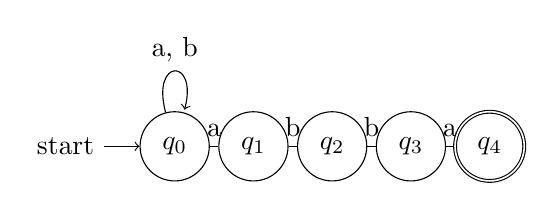
\begin{tikzpicture}
            \node[state, initial] (q0) {$q_0$};
            \node[state, right of=q0] (q1) {$q_1$};
            \node[state, right of=q1] (q2) {$q_2$};
            \node[state, right of=q2] (q3) {$q_3$};
            \node[state, right of=q3, accepting] (q4) {$q_4$};
            
            \draw   (q0) edge[above] node{a} (q1)
                    (q1) edge[above] node{b} (q2)
                    (q2) edge[above] node{b} (q3)
                    (q3) edge[above] node{a} (q4)
                    (q0) edge[loop above] node{a, b} (q0)
                    ;
        \end{tikzpicture}
    \end{figure}

    DFA:
    \begin{figure}[ht]
        \centering
        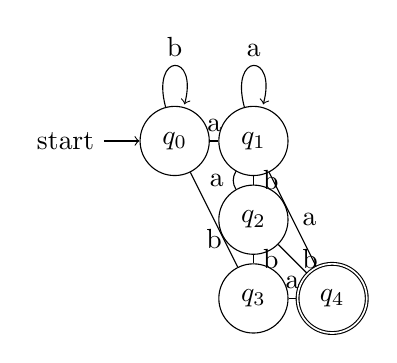
\begin{tikzpicture}
            \node[state, initial] (q0) {$q_0$};
            \node[state, right of=q0] (q1) {$q_1$};
            \node[state, below of=q1] (q2) {$q_2$};
            \node[state, below of=q2] (q3) {$q_3$};
            \node[state, right of=q3, accepting] (q4) {$q_4$};
            
            \draw   (q0) edge[above] node{a} (q1)
                    (q1) edge[right] node{b} (q2)
                    (q2) edge[right] node{b} (q3)
                    (q3) edge[above] node{a} (q4)
                    (q0) edge[loop above] node{b} (q0)
                    (q1) edge[loop above] node{a} (q1)
                    (q2) edge[left, bend left] node{a} (q1)
                    (q3) edge[below] node{b} (q0)
                    (q4) edge [right] node{a} (q1)
                    (q4) edge [right] node{b} (q2)
                    ;
        \end{tikzpicture}
    \end{figure}

    Regex: 
    $$\Sigma^*abba$$

    $\{w \in \Sigma^* ~|~ w\text{ has a single b in the 3rd place from the right}\}$

    NFA:
    \begin{figure}[ht]
        \centering
        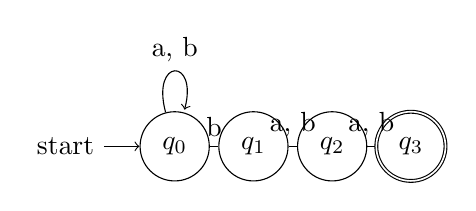
\begin{tikzpicture}
            \node[state, initial] (q0) {$q_0$};
            \node[state, right of=q0] (q1) {$q_1$};
            \node[state, right of=q1] (q2) {$q_2$};
            \node[state, right of=q2, accepting] (q3) {$q_3$};
            
            \draw   (q0) edge[above] node{b} (q1)
                    (q0) edge[loop above] node{a, b} (q0)
                    (q1) edge[above] node{a, b} (q2)
                    (q2) edge[above] node{a, b} (q3)
                    ;
        \end{tikzpicture}
    \end{figure}

    DFA:
    \begin{figure}[ht]
        \centering
        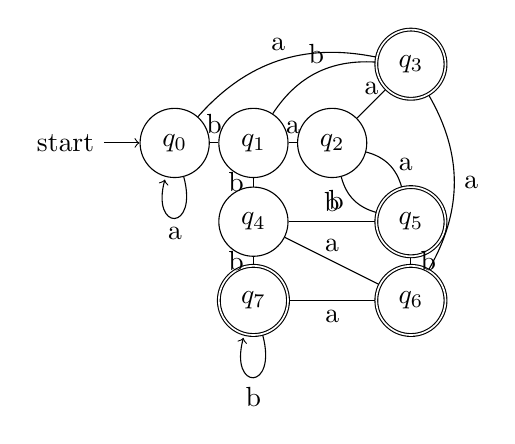
\begin{tikzpicture}
            \node[state, initial] (q0) {$q_0$};
            \node[state, right of=q0] (q1) {$q_1$};
            \node[state, right of=q1] (q2) {$q_2$};
            \node[state, right of=q2, above of=q2, accepting] (q3) {$q_3$};

            \node[state, below of=q1] (q4) {$q_4$};
            \node[state, below of=q2, right of=q2, accepting] (q5) {$q_5$};
            \node[state, below of=q5, accepting] (q6) {$q_6$};
            \node[state, below of=q4, accepting] (q7) {$q_7$};
            
            \draw   (q0) edge[loop below, below] node{a} (q0)
                    (q0) edge[above] node{b} (q1)
                    
                    (q1) edge[above] node{a} (q2)
                    (q1) edge[left] node{b} (q4)
                    
                    (q2) edge[above] node{a} (q3)
                    (q2) edge[left, bend right] node{b} (q5)
                    
                    (q3) edge[above, bend right] node{a} (q0)
                    (q3) edge[above, bend right] node{b} (q1)

                    (q4) edge[above] node{a} (q6)
                    (q4) edge[left] node{b} (q7)

                    (q5) edge[bend right, right] node{a} (q2)
                    (q5) edge[above] node{b} (q4)

                    (q6) edge[bend right, right] node{a} (q3)
                    (q6) edge[right] node{b} (q5)

                    (q7) edge[below] node{a} (q6)
                    (q7) edge[loop below, below] node{b} (q7)
                    ;
        \end{tikzpicture}
    \end{figure}

    Regex: 
    $$\Sigma^*b\Sigma\Sigma$$
    
    \item Let $L$ be a language. define $L' = \{xay \in \Sigma^*~|~ xy \in L, a \in \Sigma\}$. We take the strings in $L$, and add a single symbol anywhere in the string, even possibly at the beginning or end. Prove that if $L$ is regular, then so is $L'$.

    \solution{} Let $M = (\Sigma, Q_M, q_{M0}, \delta_M, F_M)$ be the NFA that decides $L$. Also, let $P = (\Sigma, Q_P, q_{P0}, \delta_P, F_P)$ be an exact copy of $M$ but with a new copy of the states. Now, we can create a new NFA $M'= (\Sigma, Q, q_0, \delta, F)$ to decide $L'$ as follows.

    $$\Sigma := \Sigma$$
    $$Q = Q_M \cup Q_P$$
    $$q_0 = q_{M0} \in Q_M \subset Q $$

    Then if $q_i \in Q$ and $p_i \in Q_P$ is the corresponding copy state in the NFA $P$,
    $$\delta(q_i, a) = \delta_M(q_i, a) \cup \{p_i\} $$
    and
    $$\delta(p_i, a) = \delta_P(p_i, a)$$
    Lastly, we can mark all the final states in the copy NFA $P$ as final. That is,
    $$F = F_P$$

    Note that this means a string must use a character to move from $M$ to $P$ and then end in a final state in $P$ to be accepted into the language. This means that it is a string from $L$ with an extra character injected somewhere in the string, which is $L'$ as required. Thus, we have created an NFA $M'$ that decides $L'$, meaning that $L'$ is a regular language.

    \item Prove that $\{a^nba^mb^{m+n} ~|~ m,n \in \mathbb{N}\}$ is not regular by usage of the pumping lemma.

    \solution{} Let $L$ be that language in question ($L = \{a^nba^mb^{m+n} ~|~ m,n \in \mathbb{N}\}$). 

    Assume, to the contrary, that $L$ is regular. Then, by the pumping lemma, $L$ has a pumping length $p$ and every string $s \in L$ with length $|s| \geq p$ can be divided into three parts $s=xyz$ so that $xy^iz \in L \forall i \in \mathbb{N}$, $|y|>0$, and $|xy| \leq p$.

    Consider $s=a^pba^qb^{p+q} \in L$ for any $q \in \mathbb{N}$. For our proof, lets use $q = 1$, so $s = a^pbab^{p + 1}$. Now, there is only one case to subdivide our string into three parts such that $|y| > 0$ and $|xy| \leq p$,

    $$x=a^c \qquad y=a^d \qquad z=a^{p - c - d}bab^{p+1} \qquad \text{subject to } c + d \leq p \text{ and } d > 0$$

    Now, since $y=a^d$, we should be able to pump this string so that $xy^iz \in L$ for all $i \in \mathbb{N}$. We can choose $i = 2$ and show that $xyyz \notin L$.

    $$xyyz = a^ca^da^da^{p - c - d}bab^{p+1} = a^{p + d}bab^{p + 1}$$

    Note that for the above string to be in $L$, $p + d + 1 = p + 1$, which can only be true if $d = 0$. To ensure that the length of $y$ is non-zero $d$ cannot be zero. Hence $xyyz \notin L$ and the pumping lemma does not hold. This means that $L$ is not a regular language. 

    \newpage
    
    \item Prove that a unary language is regular if and only if it is the finite union of languages whos lengths are arithmetic progressions, and a finite language.

    \solution{} First, let's define some things:

    $$\Sigma = \{a\} \qquad L_{x,y}=\{a^{xn + y} \quad \forall \quad n \in \mathbb{N}\} \text{ for some $x, y \in \mathbb{N}$ }$$

    Let's also call a language whose lengths are arithmetic progressions ($L_{x, y}$) an arithmetic language for shorthand.

    Note that an arbitrary finite union of arithmetic languages and a finite language can be represented as follows:

    $$\big(\bigcup_{k=0}^M L_{x_k, y_k}\big) \cup L_F $$

    where $M$ is the number of arithmetic languages and $L_F$ is a finite language.

    First, proving the forward read of the statement: A unary language is regular if it is the finite union of languages whose lengths are arithmetic progressions, and a finite language.

    Consider, an arbitrary $L = \big(\bigcup_{k=0}^M L_{x_k, y_k}\big) \cup L_F$. Note that $L_F$ if a finite language, and thus, must be regular as proved in question (1). Further, note that for an arbitrary arithmetic language $L_{x, y}$, we can write the following regular expression to define it: $(a^x)^*a^y$. Since this is a valid regular expression that fully decides $L_{x,y}$, $L_{x, y}$ must be regular. Then, since $L$ is a finite union of regular languages and regular languages is closed under the union, $L$ must be a regular language as well.

    Now, to prove the backward read of the statement: A unary language is a finite union of languages whose lengths are arithmetic progressions and a finite language if it is regular. In other words, it must be shown that all unary regular languages can be represented as $L = \big(\bigcup_{k=0}^M L_{x_k, y_k}\big) \cup L_F$. 

    Let the statement $T(L)$ denote that a regular language $L$ can be represented as a finite union of languages whose lengths are arithmetic progressions and a finite language. Further, let the statement $T(R)$ denote that the language $L$ a regular expression $R$ decides is true under $T(L)$.

    This proof will be done using induction over $\mathcal{L}(REX)$. First consider the base cases:

    $$\emptyset=\{\} \qquad \{\epsilon\} \qquad \{a\}$$

    Note that these are all finite languages and can thus be represented by a finite language $L_F$. Thus, $T$ is true for all three base cases. Note that $\{\epsilon\}=L_{0,0}$ and $\{a\} = L_{0,1}$ are alternate proofs of $T$ for those two base cases.

    Now, as an inductive hypothesis, let $R$ and $S$ be regular expressions that decide two potentially different regular languages such that $T(R)$ and $T(S)$ are both true. Now, to prove that $T$ extends over the space of all regular expressions, the following must be proven:

    $$T(R^*) \qquad T(RS) \qquad T(R \cup S)$$

    Since $T(R)$ and $T(S)$ are both true, the languages represented by them can be respectively written as follows:

    $$L_R = \big(\bigcup_{k=0}^{M} L_{x_k, y_k}\big) \cup L_{FR} \qquad L_S = \big(\bigcup_{k=0}^{P} L_{z_k, w_k}\big) \cup L_{FS}$$

    \textbf{Union} $T(R \cup S)$:

    Let's consider the language defined by $R \cup S$,

    $$L_R \cup L_S = \big[\big(\bigcup_{k=0}^{M} L_{x_k, y_k}\big) \cup L_{FR}\big] \cup \big[\big(\bigcup_{k=0}^{P} L_{z_k, w_k}\big) \cup L_{FS}\big] = \bigcup_{k=0}^{M+P+1} L_{a_k, b_k} \cup \big( L_{FR} \cup L_{FS} \big)$$

    where $[a_k] = [x_0, ..., x_M, z_0, ..., z_P]$ and $[b_k] = [y_0, ..., y_M, w_0, ..., w_P]$. Note that the last result above is a finite union of arithmetic languages union-ed with a finite set (since the unions of finite sets are finite). Thus, $T(R \cup S)$ is true. In other words, the set of languages that satisfy $T$ is closed under finite union.

    \textbf{Concatenation} $T(RS)$:
   
    Let's consider the language defined by $RS$,

    $$L_R L_S = \big[\big(\bigcup_{k=0}^{M} L_{x_k, y_k}\big) \cup L_{FR}\big]\big[\big(\bigcup_{k=0}^{P} L_{z_k, w_k}\big) \cup L_{FS}\big]$$

    $$ = \bigcup_{k=0}^{M} \bigcup_{l=0}^{P} L_{x_k, y_k} L_{z_l, w_l} \cup \bigcup_{k=0}^{M} L_{x_k, y_k}L_{FS} \cup \bigcup_{k=0}^{P} L_{FR}L_{z_k, w_k} \cup L_{FR}L_{FS}$$

    If we can show that all of these terms are true under $T$, then the whole expression is true under $T$ since $T$ is closed under finite union and every union here is finite.

    Consider $L_{x,y}L_{z,w}$,

    $$L_{x,y}L_{z,w} = \{a^{xn + y}a^{zm + w} | n, m \in \mathbb{N}\} = \{a^{xn + y + zm + w} | n, m \in \mathbb{N}\}$$

    Then let $m := xq + r$ by the remainder theorem where $r < x$. Since $m$ can be any natural number, $q$ and $r$ can be any natural numbers that follow the specified constraints.

    $$L_{x,y}L_{z,w} = \{a^{xn + z(xq + r) + y + w} | n, q, r \in \mathbb{N}; r < x\} = \{a^{x(n + zq) + zr + y + w} | n, q, r \in \mathbb{N}; r < x\}$$

    $$ = \bigcup_{r=0}^{x-1} \{a^{x(n + zq) + zr + y + w} | n, q \in \mathbb{N}\}$$

    Now, note that since $n$ and $q$ can be any natural numbers, $n + zq$ can produce any natural number $p$ (set $z=0$ and $n=p$). So, we can set $p = n+zq \in \mathbb{N}$:

    $$L_{x,y}L_{z,w} = \bigcup_{r=0}^{x-1} \{a^{xp + zr + y + w} | p \in \mathbb{N}\} = \bigcup_{r=0}^{x-1} L_{x, zr+y+w}$$

    The final result is a finite union ($x$ is some finite natural number) of arithmetic languages as required. So $T(L_{x,y}L_{z,w})$ is true.

    Thus, $T(L_{x_k,y_k}L_{z_k, w_k})$ is also true since all we did is add subscripts.

    Next, consider some finite language of $L_F$ concatenated with an arithmetic language $L_{x,y}$. 
    
    Note that since we are using a unary language, the order of concatenation does not that matter. That is, $L_1 L_2 = L_2 L_1$ for any two unary languages $L_1$ and $L_2$. This is because the number of characters in the string is all that really matters.

    $$L_F L_{x, y} = L_{x, y} L_F = \{a^{xn + y} \quad \forall \quad n \in \mathbb{N}\} \{ a^{c_k} | k \in \mathbb{N}, k < Q \}$$

    where we represented $L_F$ as $\{ a^{c_k} | k \in \mathbb{N}, k < Q \}$ where $\{c_0, ..., c_k, ..., c_Q\}$ is a finite set of the number of counts in each of the strings in $L_F$.

    $$L_F L_{x, y} = L_{x, y} L_F = \{a^{xn + y} \quad \forall \quad n \in \mathbb{N}\} \{ a^{c_k} | k \in \mathbb{N}, k < M \} = \{a^{xn + y} \quad \forall \quad n \in \mathbb{N}\} \big( \bigcup_{k=0}^Q \{ a^{c_k} \}\big)$$

    $$ = \bigcup_{k=0}^Q \{ a^{c_k} \} \{a^{xn + y} \quad \forall \quad n \in \mathbb{N}\} = \bigcup_{k=0}^Q  \{a^{c_k}a^{xn + y} \quad \forall \quad n \in \mathbb{N}\} = \bigcup_{k=0}^Q  \{a^{xn + y + c_k} \quad \forall \quad n \in \mathbb{N}\} $$
    
    $$ = \bigcup_{k=0}^Q L_{x, y+c_k}$$

    which is a finite union of arithmetic languages. So, $T(L_F L_{x, y})$ and $T(L_{x, y} L_F)$ are both true. Thus, $T(L_{x_k, y_k}L_{FS})$ and $T(L_{FR}L_{z_k, w_k})$ are both also true.

    Lastly, lets consider $L_{FR} L_{FS}$ where both parts are finite languages. Representing $L_{FR}$ with counts $c_k$ and $L_{FS}$ with counts $d_k$, 

    $$ L_{FR} L_{FS} = \{ a^{c_k} | k \in \mathbb{N}, k < U \} \{ a^{d_k} | k \in \mathbb{N}, k < V \} = \big( \bigcup_{k=0}^U \{ a^{c_k} \} \big) \big( \bigcup_{l=0}^V \{ a^{d_l} \} \big) = \bigcup_{k=0}^U \bigcup_{l=0}^V \{ a^{c_k + d_l} \}$$

    which is a finite union of one element sets, or just a finite set. Thus, $T(L_{FR}L_{FS})$ is also true.

    To recap,

    $$L_R L_S = \bigcup_{k=0}^{M} \bigcup_{l=0}^{P} L_{x_k, y_k} L_{z_l, w_l} \cup \bigcup_{k=0}^{M} L_{x_k, y_k}L_{FS} \cup \bigcup_{k=0}^{P} L_{FR}L_{z_k, w_k} \cup L_{FR}L_{FS}$$

    in which each term in the union is true under $T$. Then, since $T$ is closed under finite union and $L_R L_S$ is a finite union of these terms, $T(L_R L_S)$ is also true. In other words, the set of languages which is true under $T$ is closed under concatenation. 

    \textbf{Kleene Star} $T(R^*)$:

    Under unary languages, we can prove the following property:

    $$ \big( \bigcup_{k=0}^M L_k \big)^* = L_0^*\dots L_M^* $$

    Since all that matters in a unary langauge is the number of letters in the string we can prove these two expressions to be equivalent. The Kleene star implies that we can have an arbitrary amount of whatever is inside the expression. Since the union is inside the expression, we can have an arbitrary amount of elements from any of $L_0$ to $L_M$. Now, note that the order does not matter since there is only one character allowed, so we can group together everything from $L_0$, everything, from $L_1$, and so on. Essentially, we can have an arbitrary amount of each language and then order doesn't matter, so we can write it as the expression above.

    Applying this to the language represented by $R^*$

    $$ L_R^* = \big[\big(\bigcup_{k=0}^{M} L_{x_k, y_k}\big) \cup L_{FR} \big]^* = L_{x_0, y_0}^* \dots L_{x_M, y_M}^* L_{FR}^*$$

    Thus, if we can show that each term in the concatenation is true under $T$, then $L_R^*$ is true under $T$ since $T$ is closed under concatenation as we proved above.

    Let's consider $L_{x,y}^*$ first.

    $$L_{x,y}^* = \{a^{\sum_{k=0}^m (x n_k + y)} \quad \forall \quad m, n_0,\dots,n_m \in \mathbb{N}\}$$

    $$ = \{a^{x\big( \sum_{k=0}^m n_k \big )+ m y} \quad \forall \quad m, n_0,\dots,n_m \in \mathbb{N}\}$$

    Now, note that since $n_k$ is a finite arbitrary sum of natural numbers, it can represent any natural number $n$. So, we can set $n = \sum_{k=0}^T n_k$ for every $n \in \mathbb{N}$.

    $$ L_{x,y}^* = \{ a^{xn + ym} \quad \forall \quad m, n \in \mathbb{N} \} =  \{ a^{xn} \quad \forall \quad n \in \mathbb{N} \} \{ a^{ym} \quad \forall \quad m \in \mathbb{N} \} = L_{x,0} L_{y, 0}$$

    Since both $L_{x, 0}$ and $L_{y, 0}$ are both arithmetic languages, $T$ is true for both of them. Since $T$ is closed under concatenation, $T(L_{x,0} L_{y, 0}) = T(L_{x, y}^*)$ is true for an arbitrary arithmetic language $L_{x,y}$. This means that $T(L_{x_k, y_k})$ is true for all $k$. 

    Lastly, consider $L_{FR}^*$. Just like before we can write it as a finite union of single element sets with counts $c_k$.

    $$L_{FR}^* = \big[ \bigcup_{k=0}^M \{ a^{c_k} \} \big]^*$$

    Then, using the property we proved above,

    $$L_{FR}^* = \{ a^{c_0} \}^* \dots \{ a^{c_M} \}^*$$

    Note that $\{ a^{c_k} \}^* = \{a^{n c_k} \forall n \in \mathbb{N} \} = L_{c_k, 0}$, so

    $$L_{FR}^* = L_{c_0, 0}\dots L_{c_M, 0}$$

    which is a finite concatenation of arithmetic languages (which are all true under $T$). Thus, $T(L_{FR}^*)$ is true.

    To recap, 

    $$ L_R^* = L_{x_0, y_0}^* \dots L_{x_M, y_M}^* L_{FR}^*$$

    which is a finite concatenation of languages that are all proven to be true under $T$. Thus, $T(L_R^*)$ is also true.

    Finally, by induction, since we have shown the base cases are true under $T$ and any recursive definitions are also true under $T$, the entire space of languages that can be defined by regular expressions is true under $T$. This means that $T$ is true for every regular language.

    Now, that we have proven both the forward and backwards directions of the if and only if, the entire statement, a unary language is regular if and only if it is the finite union of languages whose lengths are arithmetic progressions, and a finite language, is true.
    
\end{enumerate}
\end{document}
 